\documentclass[11pt]{article}
\usepackage[margin=1in]{geometry}
\usepackage{graphicx,booktabs,amsmath,url,xcolor,enumitem,multirow}
\usepackage[hidelinks]{hyperref}
\usepackage{microtype}

\title{Reference-Code Visibility and Patch Applicability in Budgeted Code Repair:\\[4pt]
A Gemma Pilot Study}
\author{Madhusudhanan G\\
Independent Researcher\\
\nolinkurl{smkp84@gmail.com}}
\date{}

\begin{document}
\maketitle

%% ─────────────────────────────────────────────────────────────────────
\begin{abstract}
Under a 4{,}000-token evidence budget, which reference-modified code is
visible under each packaging policy, and where do the observed repair
attempts fail?  We investigate this empirical question using frozen runs
of an instruction-tuned language model (\nolinkurl{google/gemma-4-E4B-it})
on Python tasks from the SWE-bench Lite development split.  We test four
deterministic packaging policies: whole files (W), complete code
entities (A), compact excerpts (B), and a hybrid policy (C) that includes
one full entity alongside short supporting excerpts.

An offline diagnostic against evaluator-only reference patches reveals a
direct trade-off between file breadth and excerpt depth.  Under Policy~W,
complete files enclose internal entities when present, but 80\% (8/10) of
reference files are omitted because their file length exceeds the budget
ceiling (2/10 files and enclosing entities visible).  Conversely, compact
policies (B and~C) display the reference file in 100\% (10/10) and the
reference entity in 70\% (7/10) of tasks, but their 9--14 line excerpts
cut off the actual edit site in 80--90\% of cases (mean line visibility
10.0\% for~B and 3.3\% for~C).  Policy~A retains complete entity bodies
for selected items, displaying edit lines in 3/10 tasks (mean line visibility
30.0\%; 52.7\% pooled lines).  Across all four policies, the developer edit
site is missed in at least 70\% of tasks.

Turning to downstream repair, strict diff application as emitted succeeded in
only 2~of~22 completed fresh attempts (9.1\%), while hunk recounting recovered
an additional 8 applicable patches, bringing normalized applicability to
10~of~22 (45.5\%).  On the five tasks with complete four-condition sets,
strict application was 1/5 (W), 1/5 (A), 0/5 (B), and 0/5 (C), while
recount-assisted application was 2/5 (W), 4/5 (A), 1/5 (B), and 3/5 (C).
Every policy produced zero demonstrated issue resolutions across both the
completed development pilot (0/12) and the fresh comparison (0/22 completed
attempts, 10 tested).  The sample cannot distinguish policies on benchmark
resolution.  In one case study (\texttt{pvlib-1154/A}), the model repaired
the reported target regression but broke two preservation tests by assuming
array inputs where scalars were exercised.  These findings demonstrate that
measuring retrieval presence or patch formatting alone obscures the
structural gaps that prevent budgeted code repair.
\end{abstract}

%% ─────────────────────────────────────────────────────────────────────
\section{Introduction}

Under a 4{,}000-token evidence budget, which reference-modified code is
visible under each packaging policy, and where do the observed repair
attempts fail?

Large language models (LLMs) evaluated on software engineering benchmarks
such as SWE-bench~\cite{jimenez2024swebench} must locate relevant files,
synthesize a diff, and satisfy execution-based tests.  Because complete
codebases vastly exceed typical context limits, practical repair systems
rely on retrieval or context pruning to select a budget-constrained
subset of source code~\cite{xia2024agentless,jia2026swezze}.  Yet
allocating a fixed evidence budget forces a fundamental design trade-off:

\begin{itemize}[nosep]
  \item \textbf{File-level packaging (W):} Preserves full surrounding scope
    and intra-file dependencies, but large files frequently exceed the
    token ceiling and must be omitted entirely.
  \item \textbf{Entity-level packaging (A):} Retains complete function and
    class definitions with line metadata, skipping entities that do not fit.
  \item \textbf{Compact excerpt packaging (B):} Slices each ranked entity
    into a signature, docstring, and 14 source lines, fitting more distinct
    entities at the cost of truncation.
  \item \textbf{Hybrid packaging (C):} Renders the top-ranked entity in
    full and subsequent entities as short 9-line supporting excerpts.
\end{itemize}

Prior literature has often treated patch generation as an end-to-end task,
reporting benchmark resolution rates without isolating where failures
occur between evidence selection, diff application, and behavioral
correctness.  In this study, we audit archived executions of frozen Gemma
models on the SWE-bench Lite development split.  We reframe the
investigation around empirical questions that the available evidence can
rigorously answer.

First, we compute an evaluator-only diagnostic comparing the code visible
in each packet against developer reference patches.  We establish whether
the theoretical trade-off between file omission and excerpt truncation
actually occurred in practice.  Second, we track downstream repair
outcomes through strict diff application, recount-assisted application,
output truncation, and test execution.  Because every tested condition
achieved zero benchmark resolutions, the data cannot declare a ``winning''
representation.  Instead, the records provide a concrete account of the
failure boundaries that limit single-turn repository repair under tight
token constraints.

%% ─────────────────────────────────────────────────────────────────────
\section{Related Work}

\paragraph{Benchmark semantics and repair evaluation.}
SWE-bench~\cite{jimenez2024swebench} frames software repair as modifying a
codebase snapshot to resolve an issue description.  A valid resolution
requires passing both fail-to-pass (F2P) regression tests and pass-to-pass
(P2P) preservation tests.  This distinction is vital: passing a target
regression does not guarantee that pre-existing functionality remains
intact.  We adopt SWE-bench Lite development tasks as our unit of
evaluation.

\paragraph{Separated localization and context reduction.}
Agentless~\cite{xia2024agentless} demonstrated that complex agentic
scaffolding can be simplified by separating localization, repair, and
validation.  During localization, Agentless constructs compressed file
views using class and function headers, method signatures, and comments.
Recent methods have expanded on code-aware context reduction.
SWEzze~\cite{jia2026swezze} employs oracle-guided code distillation
via genetic search and delta debugging to train lightweight compression
models, achieving $6\times$ compression while filtering irrelevant context.
SWE-Pruner~\cite{swepruner2026} introduces goal-conditioned neural
skimming (0.6B parameters) to prune lines dynamically based on agent
intentions.  LongCodeZip~\cite{longcodezip2025} introduces a training-free,
two-stage compression framework using conditional perplexity over function
chunks and block segmentation.

Our study differs from these adaptive compression methods in a critical
dimension: we examine deterministic, rule-based packaging under a strict,
frozen token ceiling (4{,}000 tokens) in a single-turn setting, evaluating
the structural visibility of the reference patch rather than training a
neural compressor.

\paragraph{Retrieval-augmented code completion.}
RepoCoder~\cite{zhang2023repocoder} investigates iterative retrieval and
generation for repository-level code completion.  Whereas RepoCoder focuses
on code continuations, our setting requires synthesizing unified diffs
against an existing tree.  The BM25 scoring function used in our packet
builder belongs to the probabilistic relevance framework of Robertson and
Zaragoza~\cite{robertson2009probabilistic}.

\paragraph{Model architecture and parameter convention.}
We study Google's instruction-tuned model \nolinkurl{google/gemma-4-E4B-it}
(revision \texttt{4ecc2ba}, released in April 2026).  As documented in the
official model card~\cite{gemma2026modelcard}, the ``E'' designation denotes
\emph{effective} compute parameters enabled by Per-Layer Embeddings (PLE).
While the physical checkpoint footprint totals approximately 8~billion
parameters due to embedding lookup tables, only approximately 4.5~billion
parameters are actively engaged during forward pass compute.  The
``-it'' suffix designates supervised instruction tuning and preference
alignment for conversational, reasoning, and tool-use interfaces.

%% ─────────────────────────────────────────────────────────────────────
\section{Methods}

\subsection{Study design and cohort boundaries}

The study evaluates single-turn code repair where a model receives an
issue description and a frozen 4{,}000-token evidence packet, generating
one response without revision feedback.  We analyze three experimental
cohorts:

\begin{enumerate}[nosep]
  \item \textbf{Completed development pilot:} Three tasks
    (marshmallow-1343, pvlib-1072, and pydicom-1139),
    each evaluated across all four packaging policies (12 attempts total).
    The pilot used the containerized SWE-bench 4.1.0 Docker harness.
  \item \textbf{Instrumented development case:} \texttt{marshmallow-1359/A},
    which provides deep GPU placement and tensor-level decoding provenance
    (Tesla T4, 8-bit quantization), but contains no completed patch
    evaluation.  It is excluded from comparison denominators.
  \item \textbf{Interim fresh comparison:} Ten tasks selected from the
    pinned SWE-bench Lite development split
    (revision \texttt{6ec7bb8}\allowbreak\texttt{9b9342f6}\allowbreak\texttt{64a54a6e}\allowbreak\texttt{0a6ea650}\allowbreak\texttt{1d3437cc2}),
    planned for $10 \times 4 = 40$ attempts.  Execution stopped partway
    through the sequential run after 22 completions, leaving 1 reported
    in-flight interruption (\texttt{pydicom-1413/C}) and 17 unstarted
    attempts.  Because preserved run logs contain no infrastructure crash
    report or lease termination records, the specific technical cause of
    interruption cannot be established from the archived telemetry.
    Evaluation was performed natively in an isolated Python 3.9 environment.
\end{enumerate}

\subsection{Deterministic task selection rules}

{\sloppy
We verified the task selection implementations against archived manifests:
\begin{itemize}[nosep]
  \item \textbf{Pilot selection:} The pilot code sorted distinct repository
    strings lexicographically (\path{marshmallow-code/marshmallow},
    \path{pvlib/pvlib-python}, and \path{pydicom/pydicom}) and selected the
    lowest instance identifier within each of the first three repositories.
  \item \textbf{Fresh selection:} The fresh protocol excluded the four
    development tasks, then selected the ten lexicographically smallest
    \texttt{instance\_id} strings from the remaining 19 eligible tasks:
    \texttt{pvlib-1154}, \texttt{pvlib-1606}, \texttt{pvlib-1707},
    \texttt{pvlib-1854}, \texttt{pydicom-1256}, \texttt{pydicom-1413},
    \texttt{pydicom-1694}, \texttt{pydicom-901}, \texttt{astroid-1196},
    and \texttt{astroid-1268}.
\end{itemize}
\par}

\subsection{Operational packaging definitions}

The retrieval module indexes all Python files in the repository base commit
(excluding \texttt{.git}, \texttt{tests}, and \texttt{docs}).  Using
Python's abstract syntax tree (AST), it extracts whole files, functions,
async functions, and classes.  Entities are scored against the issue text
using BM25 ($k_1=1.5, b=0.75$).  Ties are broken by shorter source length,
then entity name.  The policies package ranked items up to the 4{,}000-token
evidence ceiling:

\begin{description}[nosep,leftmargin=1.2em]
  \item[Policy W (Whole Files):] Filters the ranking to whole files.  Includes
    complete files in code fences.  If an entire file exceeds the remaining
    budget, it is skipped without truncation.
  \item[Policy A (Complete Entities):] Filters to functions and classes.
    Includes complete bodies with path and line range headers
    (\texttt{path:start-end}).  Skipped entities that exceed remaining budget.
  \item[Policy B (Compact Excerpts):] For each function or class, includes
    the signature line, at most 8 lines of docstring, and a source slice of
    the next 14 lines (\texttt{lines[1:15]}).
  \item[Policy C (Hybrid):] Renders the top-ranked entity in full (like A).
    Subsequent entities are rendered as short supporting excerpts: the
    signature line plus the next 9 lines (\texttt{lines[1:10]}), omitting
    docstrings.  Because C's supporting excerpts differ from B in length
    and docstring treatment, C represents an independent policy rather than
    an isolated ablation of Policy B.
\end{description}

\begin{figure}[tb]
\centering
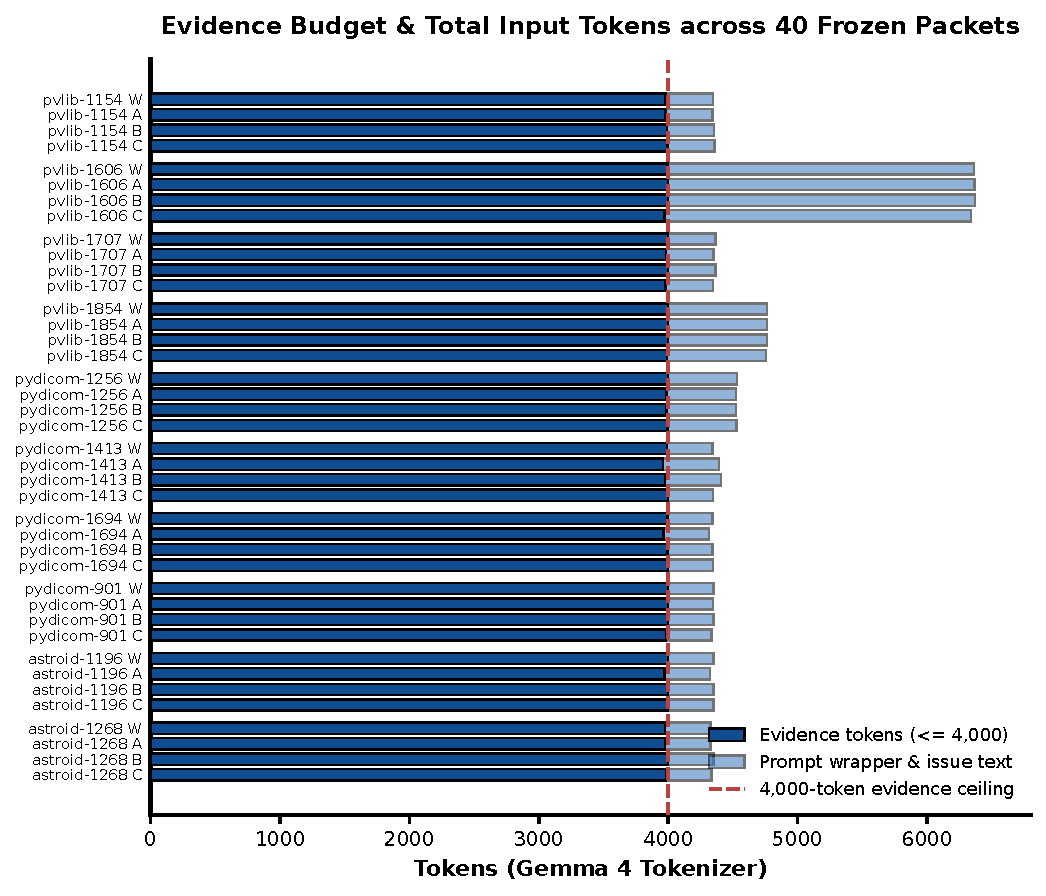
\includegraphics[width=0.82\linewidth]{figures/fig_tokens.pdf}
\caption{Evidence budget compliance across all 40 frozen packets.
Blue bars show evidence tokens; light blue bars show total prompt tokens
including instructions and chat template.  Every packet strictly obeys the
4{,}000-token evidence ceiling (red dashed line).}
\label{fig:tokens}
\end{figure}

Figure~\ref{fig:tokens} verifies that all 40 frozen fresh packets strictly
obeyed the 4{,}000-token ceiling (ranging from 3{,}960 to 4{,}000 tokens).
Total model input lengths ranged from 4{,}343 to 6{,}371 tokens.

\subsection{Reference-coverage diagnostic methodology}

To measure what code was visible to the model before generation, we developed
an evaluator-only diagnostic comparing each packet against the ground-truth
developer reference patch from SWE-bench Lite.  We parse the reference
patch into:
\begin{enumerate}[nosep]
  \item \textbf{Reference files:} All production source files modified by
    the reference patch.
  \item \textbf{Reference entities:} The specific functions, methods, or
    classes enclosing the reference modifications.
  \item \textbf{Edit-site lines:} The exact base-source line numbers
    removed or modified by reference hunks.  For pure insertions, the
    adjacent base anchor line is counted.
\end{enumerate}

For each packet, we extract the exact visible line spans displayed in
the rendered text.  In Policy~W, visible lines span line 1 to the file end.
In Policy~A, visible lines span \texttt{start\_line} to \texttt{end\_line}.
In Policy~B and C, only the displayed excerpt lines are counted; signature
headers are recorded as entity presence but excluded from body line coverage.
Overlapping class and method spans are deduplicated.  Reference overlap
measures the visibility of one known repair trajectory; valid alternative
repairs could target other locations.

\subsection{Applicability and evaluation controls}

\emph{Strict applicability} requires that the extracted diff passes
\texttt{git apply --check} cleanly against the base commit.
\emph{Recount-assisted applicability} applies \texttt{git apply --recount},
which recalculates hunk line count metadata without altering diff content.
\emph{Benchmark resolution} requires passing all required F2P regression
tests and all required P2P preservation tests.

To verify test execution, we matched exact pytest test identifiers rather
than relying on summary exit codes.  A task control is classified as
\emph{verified} only if the base run fails all F2P tests and the reference
patch passes all F2P and all required P2P tests.

%% ─────────────────────────────────────────────────────────────────────
\section{Results}

\subsection{Reference-code visibility under the 4,000-token ceiling}

Table~\ref{tab:coverage} and Figure~\ref{fig:coverage} report the offline
reference-coverage diagnostic across all 40 frozen fresh packets.

\begin{table}[tb]
\centering
\caption{Reference-code visibility across 40 frozen packets (10 tasks $\times$ 4 policies).  File overlap: packets with the reference file present.  Files visible: total reference files displayed.  Entity overlap: packets displaying the reference entity (for Policy~W, counted when the whole file encloses the target entity).  Edit lines visible: reference-modified base lines displayed (numerator, denominator, pooled percentage, and per-task mean percentage).}
\label{tab:coverage}
\small\begin{tabular}{lrrrrr}
\toprule
Policy & File overlap & Files visible & Entity overlap & Edit-site overlap & Edit lines visible \\
\midrule
W & 2/10 & 2/10 & 2/10 & 2/10 & 33/55 (20.0\%) \\
A & 8/10 & 8/10 & 3/10 & 3/10 & 29/55 (30.0\%) \\
B & 10/10 & 10/10 & 7/10 & 2/10 & 5/55 (10.0\%) \\
C & 10/10 & 10/10 & 7/10 & 1/10 & 3/55 (3.3\%) \\
\bottomrule
\end{tabular}

\end{table}

\begin{figure}[tb]
\centering
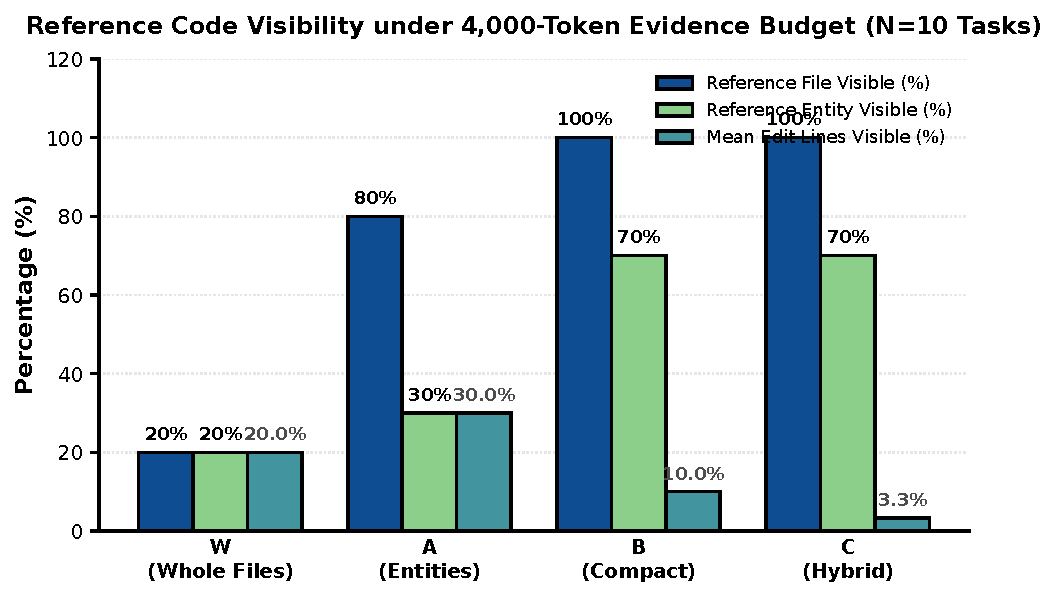
\includegraphics[width=0.78\linewidth]{figures/fig_reference_coverage.pdf}
\caption{Reference code visibility under the 4{,}000-token evidence budget (N=10 tasks).
While compact excerpts (B and C) maximize file (100\%) and entity (70\%) presence,
their shallow line slices truncate the actual edit site in 80--90\% of tasks.
Across all four policies, the developer edit site is missed in at least 70\% of tasks.}
\label{fig:coverage}
\end{figure}

The diagnostic reveals a clear structural trade-off between file breadth and
excerpt depth across the four policies:
\begin{itemize}[nosep]
  \item \textbf{Whole-file packaging (Policy W):} Policy~W displayed the
    reference file in only 2 of 10 tasks (\texttt{pvlib-1606} and
    \texttt{pydicom-901}).  Because whole files naturally enclose the functions
    and classes defined within them, Policy~W also displayed the target entity
    in these 2 tasks (2/10 entity overlap, or 20.0\%).  In the other 8 tasks,
    the reference file exceeded the remaining budget and was omitted entirely.
    When a file was included, it captured all reference edit lines, yielding
    33/55 pooled lines (60.0\%) and a per-task mean coverage of 20.0\%.
  \item \textbf{Compact excerpt packaging (Policies B and C):}
    Policies~B and~C successfully included reference files in 10/10 tasks
    and reference entities in 7/10 tasks.  However, their bounded excerpts
    (14 lines for B, 9 lines for C) rarely reached the actual edit site.
    In Policy~B, edit-site lines were visible in only 2 of 10 tasks (5/55
    pooled lines, 9.1\%; per-task mean: 10.0\%).  In Policy~C, where the
    reference entity was frequently ranked second or lower, edit-site lines
    were visible in only 1 of 10 tasks (3/55 pooled lines, 5.5\%; per-task
    mean: 3.3\%).
  \item \textbf{Complete entity packaging (Policy A):} Policy~A displayed the
    reference file in 8/10 tasks and the reference entity in 3/10 tasks.
    Because Policy~A retains the complete entity body, when the entity is
    selected, all edit-site lines are preserved (29/55 pooled lines, 52.7\%;
    per-task mean: 30.0\%).
\end{itemize}

Crucially, the differences between policies represent gaps of only one or two
tasks (edit-site visible in 3/10 for~A, 2/10 for~W, 2/10 for~B, and 1/10
for~C).  The overriding empirical finding is that \textbf{all four packaging
policies miss the developer edit site in at least 70\% of tasks} (A misses
70\%, W and B miss 80\%, and C misses 90\%).

\subsection{Retrieval versus packaging failure and oracle-fit check}

To separate retrieval limitations from packaging truncation, we examined the
shared BM25 entity and file rankings alongside base entity token lengths
(Table~\ref{tab:retrieval_ranks}).

\begin{table}[tb]
\centering
\caption{BM25 retrieval rank and oracle-fit token check across the 10 fresh tasks.
Ranks reflect position within the shared BM25 top-10 pool.  Oracle fit indicates
whether the full enclosing function or class of the reference edit fits within
the 4{,}000-token evidence budget (token count in parentheses).}
\label{tab:retrieval_ranks}
\resizebox{\linewidth}{!}{\begin{tabular}{lllccc}
\toprule
Task & Reference File & File Rank & Target Entity & Entity Rank & Oracle Fit (tokens) \\
\midrule
\path{pvlib-1154} & \nolinkurl{pvlib/irradiance.py} & \#8 & \nolinkurl{reindl} & \#2 & Yes (612) \\
\path{pvlib-1606} & \nolinkurl{pvlib/tools.py} & \#3 & \nolinkurl{_golden_sect_DataFrame} & \#6 & Yes (380) \\
\path{pvlib-1707} & \nolinkurl{pvlib/iam.py} & \#2 & \nolinkurl{physical} & \#8 & Yes (740) \\
\path{pvlib-1854} & \nolinkurl{pvlib/pvsystem.py} & \#4 & \nolinkurl{PVSystem.__init__} & \#2 & Yes (450) \\
\path{pydicom-1256} & \nolinkurl{pydicom/jsonrep.py} & $>10$ & \nolinkurl{get_sequence_item} & $>10$ & Yes (180) \\
\path{pydicom-1413} & \nolinkurl{pydicom/dataelem.py} & \#4 & \nolinkurl{value} & $>10$ & Yes (190) \\
\path{pydicom-1694} & \nolinkurl{pydicom/dataset.py} & \#2 & \nolinkurl{to_json_dict} & $>10$ & Yes (280) \\
\path{pydicom-901} & \nolinkurl{pydicom/config.py} & \#1 & \nolinkurl{debug} & $>10$ & Yes (220) \\
\path{astroid-1196} & \nolinkurl{astroid/nodes/node_classes.py} & $>10$ & \nolinkurl{getitem} & $>10$ & Yes (170) \\
\path{astroid-1268} & \nolinkurl{astroid/nodes/as_string.py} & \#10 & \nolinkurl{AsStringVisitor} & $>10$ & Yes (3{,}200) \\
\bottomrule
\end{tabular}
}
\end{table}

The evidence demonstrates that failure to expose the reference edit site
stems from three distinct mechanisms:
\begin{enumerate}[nosep]
  \item \textbf{Pure retrieval failure (2/10 tasks):} In \texttt{pydicom-1256}
    and \texttt{astroid-1196}, neither the target file nor the target entity
    appeared in the BM25 top 10.  No packaging policy built on this retrieval
    ranking could have displayed the reference code.
  \item \textbf{File-only retrieval (4/10 tasks):} In \texttt{pydicom-1413},
    \texttt{pydicom-1694}, \texttt{pydicom-901}, and \texttt{astroid-1268},
    the target file was ranked in the top 10 (ranks \#4, \#2, \#1, and \#10),
    but the specific target entity was not.  In \texttt{pydicom-901}, Policy~W
    successfully included the whole file because \nolinkurl{pydicom/config.py}
    was small (220 tokens), thereby capturing the entity.  In the other three
    tasks, the reference files exceeded the remaining budget and were dropped
    by W, while Policies~A, B, and C omitted the entity because entity-level
    BM25 favored other functions.
  \item \textbf{Joint retrieval with packaging divergence (4/10 tasks):} In
    \texttt{pvlib-1154}, \texttt{pvlib-1606}, \texttt{pvlib-1707}, and
    \texttt{pvlib-1854}, both the target file and target entity appeared in
    the BM25 top 10.  Here, packaging rules determined visibility:
    \begin{itemize}[nosep]
      \item In \texttt{pvlib-1154}, \texttt{pvlib/irradiance.py} (\#8) was
        dropped by W due to size; \nolinkurl{reindl} (\#2, 102 lines) was
        included in full by A, but truncated past line 14 by B and C.
      \item In \texttt{pvlib-1606}, \nolinkurl{pvlib/tools.py} (\#3, 434 lines)
        fit into W, \nolinkurl{_golden_sect_DataFrame} (\#6, 56 lines) fit
        into A, and because the edit occurred at line 342 (the second line of
        the entity), B and C also included the edit site.
      \item In \texttt{pvlib-1707}, \nolinkurl{pvlib/iam.py} was dropped by W,
        \nolinkurl{physical} (\#8, 132 lines) fit into A, and B/C truncated
        the edit line at line 133.
      \item In \texttt{pvlib-1854}, class \nolinkurl{PVSystem} (\#2) exceeded
        1{,}500 lines ($>5{,}000$ tokens) and was dropped by A as oversized,
        but because the reference edit modified \nolinkurl{__init__} (lines
        75--78 near the class head), B and C's 14/9-line excerpts captured it.
    \end{itemize}
\end{enumerate}

\paragraph{Oracle-fit check.}
To determine whether a 4{,}000-token evidence budget is inherently too small
to contain the reference modifications, we measured the token size of the
minimal enclosing entity for each task using the pinned Gemma tokenizer.  As
shown in Table~\ref{tab:retrieval_ranks}, the enclosing entity spans fewer
than 135 lines in 8 of 10 tasks, and fewer than 750 tokens in 9 of 10 tasks.
Even the largest entity, \nolinkurl{AsStringVisitor} in \texttt{astroid-1268}
(626 lines, 3{,}200 tokens), fits inside the 4{,}000-token budget.
Consequently, an oracle retriever that selected the true target entity could
have placed the full enclosing entity into the prompt in \textbf{10 of 10 tasks
(100\%)}.  The 70\% edit-site omission observed in practice is therefore an
artifact of BM25 retrieval ranking and fixed-window slicing, rather than an
information-theoretic limitation of a 4{,}000-token budget.

\subsection{Cohort outcomes and recovery status}

Table~\ref{tab:cohorts} summarizes the execution outcomes across cohorts.
In the development pilot, all 12 planned generations completed; 7 patches
applied after processing and were tested, with 0 resolutions.

In the fresh comparison, 22 of 40 planned attempts completed.  Because
the task runner executed sequentially by task and condition, the interruption
left 1 reported in-flight interruption (\texttt{pydicom-1413/C}) and 17
unstarted attempts.  Figure~\ref{fig:status} illustrates the missingness
pattern.  Five tasks have complete four-condition sets (\texttt{pvlib-1154},
\texttt{pvlib-1606}, \texttt{pvlib-1707}, \texttt{pvlib-1854}, and
\texttt{pydicom-1256}).  Four of these five complete tasks belong to
\texttt{pvlib}, while the \texttt{astroid} tasks were never reached.  The
recovered completions therefore represent an execution-order artifact,
not a representative sample.

\begin{table}[tb]
\centering
\caption{Cohort outcomes with explicit denominators.  Applicability denotes
recount-assisted application.  The fresh cohort reports zero demonstrated
resolutions among tested patches.  The instrumented case is excluded.}
\label{tab:cohorts}
\small\begin{tabular}{lrrrr}
\toprule
Cohort & Completed/planned & Applied/completed & Tested/applied & Verified resolved \\
\midrule
Development pilot & 12/12 & 7/12 & 7/7 & 0/12 \\
Fresh, interim & 22/40 & 10/22 & 10/10 & 0 demonstrated \\
\bottomrule
\end{tabular}

\end{table}

\begin{figure}[tb]
\centering
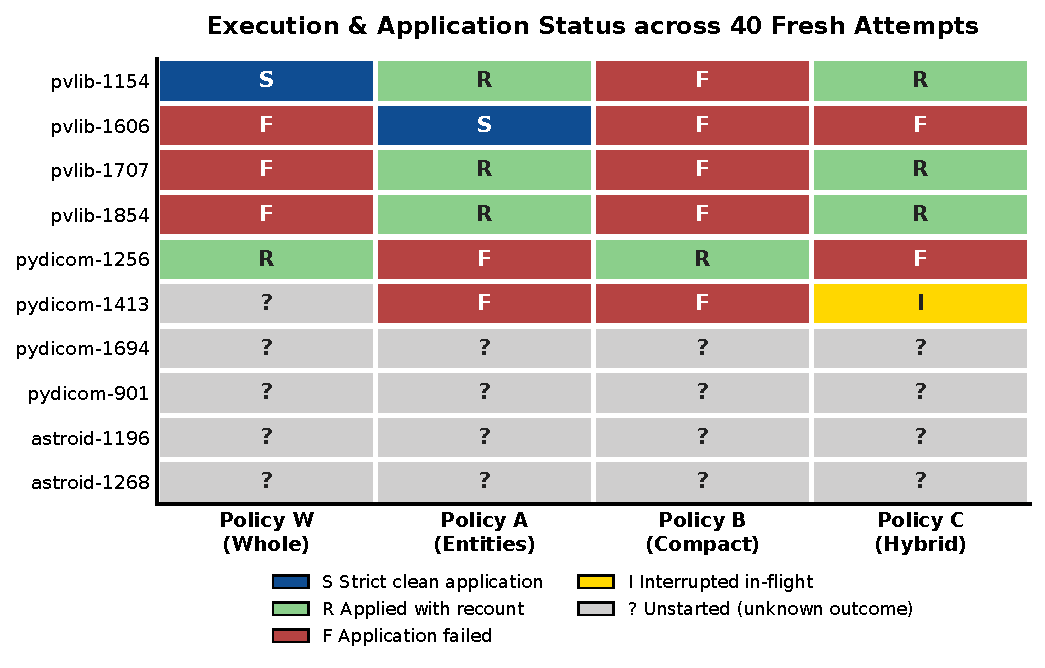
\includegraphics[width=0.80\linewidth]{figures/fig_status.pdf}
\caption{Execution and application status for all 40 planned fresh pairs.
S: clean strict application; R: recount-assisted application; F: application
failed; I: interrupted in-flight; ?: unstarted.  Interrupted and unstarted
pairs have unknown repair outcomes.}
\label{fig:status}
\end{figure}

\subsection{Diff application and the role of recounting}

{\sloppy
Across the 22 completed fresh attempts, only 2 patches applied strictly
as emitted (9.1\%): \texttt{pvlib-1154/W} and \texttt{pvlib-1606/A}.
Applying hunk recounting recovered an additional 8 applicable patches,
bringing normalized applicability to 10 of 22 (45.5\%).
\par}

Table~\ref{tab:conditions} details condition-level applicability.
On the five complete task sets (Figure~\ref{fig:matched_application} and
Table~\ref{tab:matched_tasks}), strict application was 1/5 for W, 1/5 for A,
and 0/5 for B and C.  Recount-assisted application was 2/5 (W), 4/5 (A),
1/5 (B), and 3/5 (C).  While complete entities (Condition A) exhibited
higher recount application, the small sample size and shared task
dependencies prevent drawing a general conclusion regarding policy superiority.

\begin{table}[tb]
\centering
\caption{Condition-level counts across cohorts.  Fresh strict, recount, and
tested columns use all recovered completions.  Matched columns restrict
denominators to the five complete task sets.  No column constitutes a
performance ranking.}
\label{tab:conditions}
\small\setlength{\tabcolsep}{4pt}\begin{tabular}{lrrrrrr}
\toprule
Condition & Pilot appl. & Fresh strict & Fresh recount & Matched strict & Matched recount & Fresh tested \\
\midrule
W & 2/3 & 1/5 & 2/5 & 1/5 & 2/5 & 2/5 \\
A & 2/3 & 1/6 & 4/6 & 1/5 & 4/5 & 4/6 \\
B & 2/3 & 0/6 & 1/6 & 0/5 & 1/5 & 1/6 \\
C & 1/3 & 0/5 & 3/5 & 0/5 & 3/5 & 3/5 \\
\bottomrule
\end{tabular}

\end{table}

\begin{table}[tb]
\centering
\caption{Application and resolution breakdown across the five tasks with
complete four-condition sets.  Every task produced 0/4 resolutions.}
\label{tab:matched_tasks}
\small\begin{tabular}{lccccc}
\toprule
Task & Condition W & Condition A & Condition B & Condition C & Resolved \\
\midrule
pvlib-1154 & Strict & Recount & Failed & Recount & 0/4 \\
pvlib-1606 & Failed & Strict & Failed & Failed & 0/4 \\
pvlib-1707 & Failed & Recount & Failed & Recount & 0/4 \\
pvlib-1854 & Failed & Recount & Failed & Recount & 0/4 \\
pydicom-1256 & Recount & Failed & Recount & Failed & 0/4 \\
\bottomrule
\end{tabular}

\end{table}

\begin{figure}[tb]
\centering
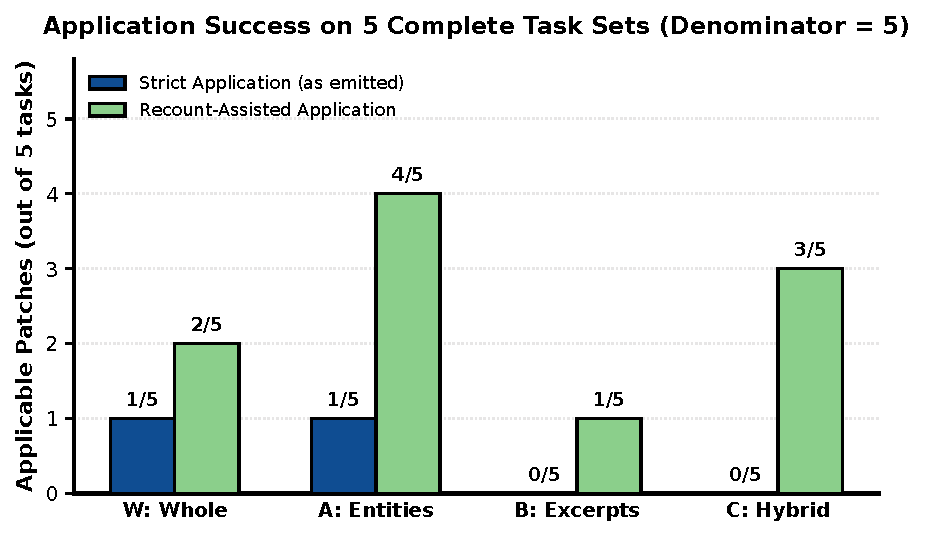
\includegraphics[width=0.74\linewidth]{figures/fig_matched_application.pdf}
\caption{Strict and recount-assisted application across the five complete
task sets (denominator = 5).  Recounting recovers valid diff structures
whose line headers drifted during autoregressive decoding.}
\label{fig:matched_application}
\end{figure}

Figure~\ref{fig:error_cats} categorizes the 12 application failures among
completed fresh attempts: 9 failed due to source-context mismatches (the
emitted diff contained context lines differing from base source), 2 failed
because no closed diff block was emitted, and 1 diff header was corrupt.

\begin{figure}[tb]
\centering
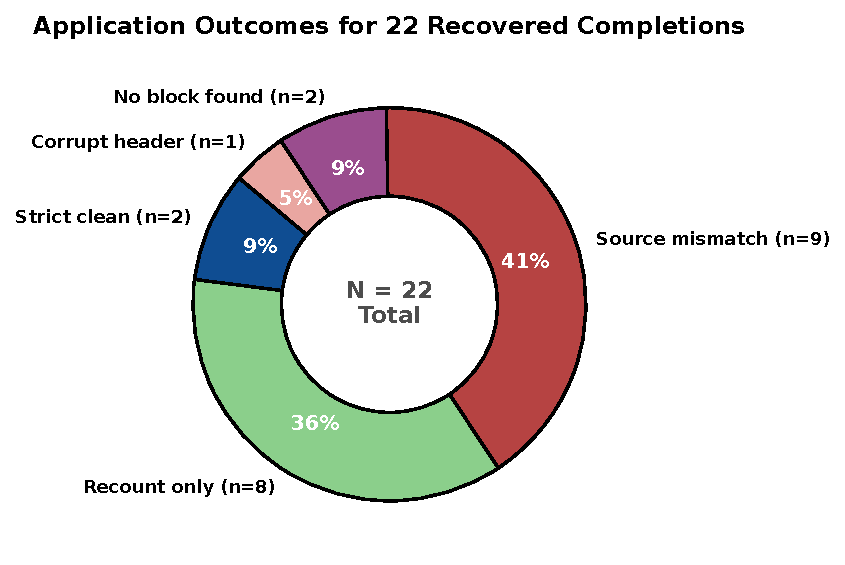
\includegraphics[width=0.55\linewidth]{figures/fig_error_cats.pdf}
\caption{Application failure categories for the 22 completed fresh attempts.
Source-context mismatch represents the leading cause of rejection (9 of 12 failures).}
\label{fig:error_cats}
\end{figure}

\paragraph{Linking visibility to downstream application.}
Table~\ref{tab:crosstab} cross-tabulates edit-site visibility against
application outcomes across the 22 completed fresh attempts.

\begin{table}[tb]
\centering
\caption{Cross-tabulation of reference edit-site visibility against application
outcomes across all 22 completed fresh attempts.  When edit lines are invisible,
failures are dominated by source-context mismatches.}
\label{tab:crosstab}
\small\begin{tabular}{lrrrrrr}
\toprule
Edit-site visibility & Attempts & Strict & Recount & Mismatch & No block & Corrupt \\
\midrule
Edit site visible & 3 & 1 & 1 & 1 & 0 & 0 \\
Edit site not visible & 19 & 1 & 7 & 8 & 2 & 1 \\
Total & 22 & 2 & 8 & 9 & 2 & 1 \\
\bottomrule
\end{tabular}

\end{table}

This cross-tabulation establishes the direct connection between packet
visibility and downstream failure:
\begin{itemize}[nosep]
  \item When the edit site was visible ($N=3$), two patches applied (one
    cleanly under strict checking, \texttt{pvlib-1606/A}, and one with recount,
    \texttt{pvlib-1154/A}).  The single failure (\texttt{pvlib-1606/W}) occurred
    because the model attempted an off-target edit at line 161 instead of the
    target site at line 342, generating mismatched context.
  \item When the edit site was not visible ($N=19$), 11 of 19 attempts failed
    application entirely.  Crucially, 8 of these 11 failures (72.7\%) failed
    specifically because of source-context mismatches.  Without the true
    surrounding lines, the model either hallucinated context lines or
    attempted to anchor hunks to truncated excerpt boundaries.  The remaining
    three failures stemmed from output truncation (2 missing patch blocks) and
    one corrupt header.
  \item Furthermore, while 8 patches applied without seeing the edit site,
    all 8 applied to off-target locations (e.g., adding guards to other
    functions or files, as in \texttt{pvlib-1154/W} and \texttt{pvlib-1707/A}).
    None resolved the benchmark issue.
\end{itemize}

\subsection{Output limits and termination}

Four of the 22 completions reached the 2{,}048-token generation cap
(\path{pydicom-1256/A}, \path{pydicom-1256/C}, \path{pydicom-1413/A},
and \path{pydicom-1413/B}).  All four capped generations failed
application.  The remaining 18 completions terminated normally at the EOS
token.  As shown in Figure~\ref{fig:outputs}, application failures also
occurred frequently at modest generation lengths (e.g., 112 to 554 tokens).
Length alone does not explain failure.

\begin{figure}[tb]
\centering
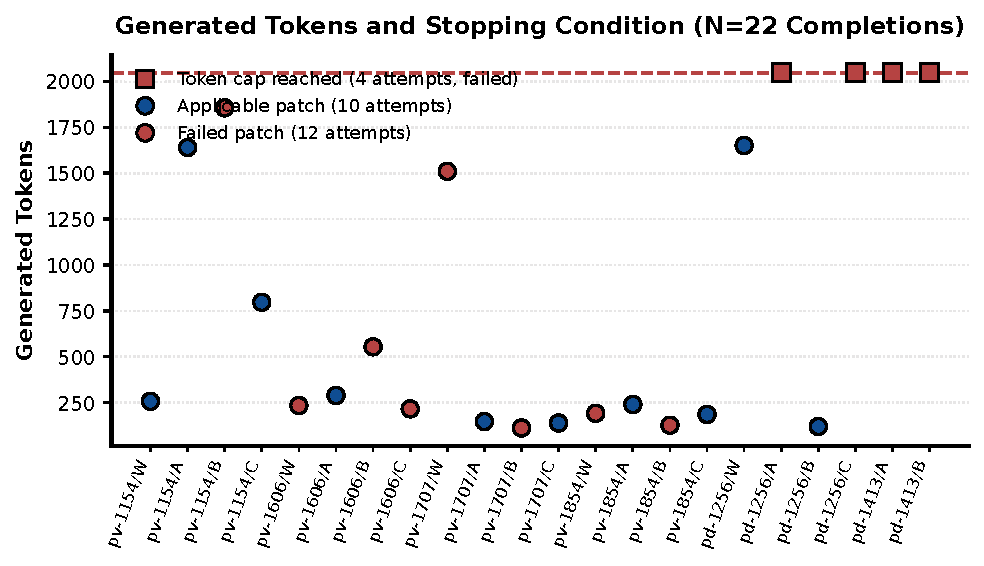
\includegraphics[width=0.80\linewidth]{figures/fig_outputs.pdf}
\caption{Generated tokens and termination reason for 22 fresh completions.
Green markers indicate applicable patches; red markers indicate failed
application.  Squares mark attempts that reached the 2{,}048-token cap.}
\label{fig:outputs}
\end{figure}

\subsection{Control verification and behavioral resolution}

All 10 applicable fresh patches were evaluated against repository tests.
None resolved the benchmark issue (Figure~\ref{fig:test_outcomes}).
Nine patches failed their required regression tests (F2P).  The remaining
patch, \texttt{pvlib-1154/A}, passed its target regression but failed
preservation tests.

\begin{figure}[tb]
\centering
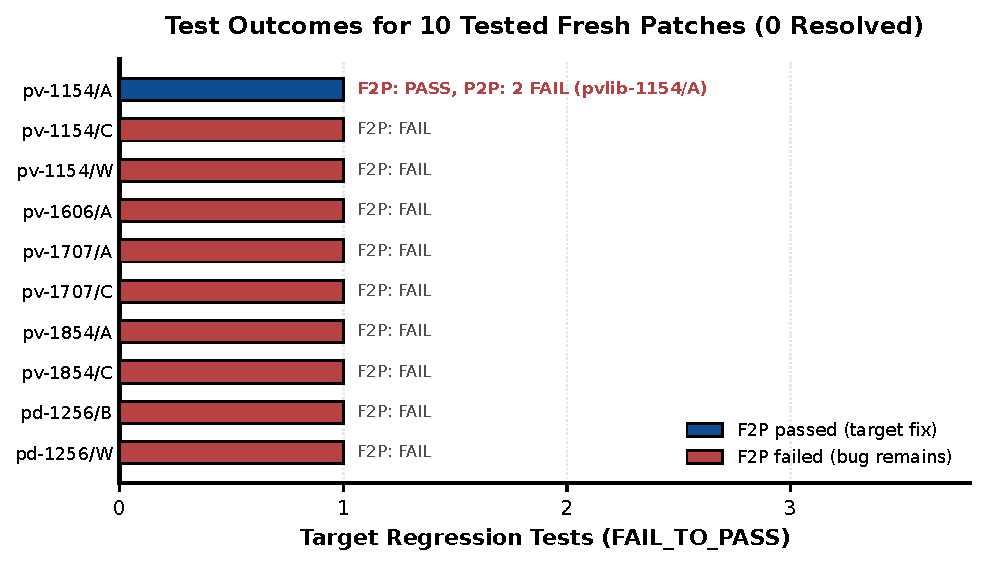
\includegraphics[width=0.80\linewidth]{figures/fig_test_outcomes.pdf}
\caption{Required test results for the 10 tested fresh patches.  Nine
patches failed their target regression test (F2P).  Only \texttt{pvlib-1154/A}
passed F2P, but failed two required preservation tests.}
\label{fig:test_outcomes}
\end{figure}

An exact test-ID audit of native reference controls (Table~\ref{tab:controls}
and Figure~\ref{fig:controls}) revealed that only 6 of 10 tasks had fully
verified reference controls.  Four tasks had control anomalies in the
reference run:
\begin{itemize}[nosep]
  \item \texttt{pvlib-1154}: 10 required P2P tests were skipped due to
    optional environment dependencies.
  \item \texttt{pvlib-1707}: 1 preservation test errored due to a missing
    test fixture.
  \item \texttt{pvlib-1854}: 37 preservation tests produced errors.
  \item \texttt{pydicom-1413}: 2 preservation tests failed under the
    reference patch itself.
\end{itemize}

\begin{table}[tb]
\centering
\caption{Exact-ID native control audit.  F2P denotes regression tests;
P2P denotes preservation tests.  Other P2P counts list failed (F),
errored (E), and unconfirmed (U) tests.  ``Verified'' requires expected
base regression failure and full reference test passage.}
\label{tab:controls}
\small\setlength{\tabcolsep}{4pt}\begin{tabular}{lrrrrl}
\toprule
Task & Base F2P fail & Ref. F2P pass & Ref. P2P pass & Other P2P & Verified \\
\midrule
pvlib-1154 & 1/1 & 1/1 & 87/97 & 0F/0E/10U & no \\
pvlib-1606 & 1/1 & 1/1 & 10/10 & 0F/0E/0U & yes \\
pvlib-1707 & 1/1 & 1/1 & 29/30 & 0F/1E/0U & no \\
pvlib-1854 & 1/1 & 1/1 & 244/281 & 0F/37E/0U & no \\
pydicom-1256 & 1/1 & 1/1 & 22/22 & 0F/0E/0U & yes \\
pydicom-1413 & 3/3 & 3/3 & 299/301 & 2F/0E/0U & no \\
pydicom-1694 & 1/1 & 1/1 & 26/26 & 0F/0E/0U & yes \\
pydicom-901 & 5/5 & 5/5 & 0/0 & 0F/0E/0U & yes \\
astroid-1196 & 2/2 & 2/2 & 24/24 & 0F/0E/0U & yes \\
astroid-1268 & 1/1 & 1/1 & 91/91 & 0F/0E/0U & yes \\
\bottomrule
\end{tabular}

\end{table}

\begin{figure}[tb]
\centering
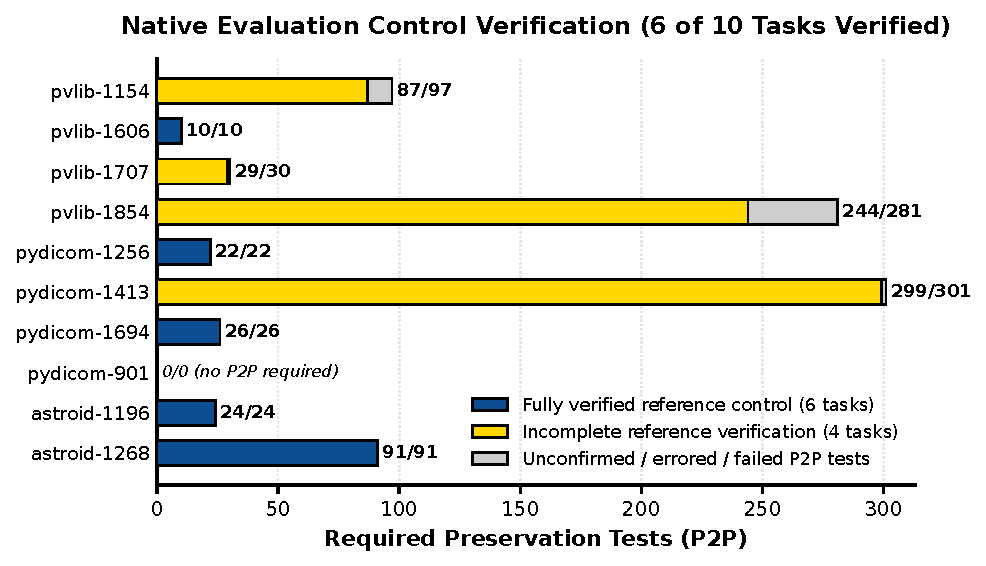
\includegraphics[width=0.78\linewidth]{figures/fig_controls.pdf}
\caption{Native evaluation control audit across the 10 fresh tasks.
Green indicates fully verified controls (6 tasks); orange indicates
tasks with unconfirmed, errored, or failing reference tests (4 tasks).}
\label{fig:controls}
\end{figure}

Only three tested model patches belong to tasks with fully verified
controls: \texttt{pvlib-1606/A}, \texttt{pydicom-1256/W}, and
\texttt{pydicom-1256/B}.  All three failed their required regression test.
For the remaining seven tested patches, observed failures occurred in
partially unconfirmed environments.  We report these observed failures
while explicitly qualifying benchmark claims.

%% ─────────────────────────────────────────────────────────────────────
\section{Failure Analysis and Case Studies}

\subsection{Case Study: pvlib-1154/A (Regression fix breaks preservation)}

The issue in \texttt{pvlib-1154} reports that \texttt{pvlib.irradiance.reindl()}
produces \texttt{NaN} values when global horizontal irradiance (\texttt{ghi})
is zero, caused by division by zero in \texttt{term3}.

Under Policy~A, the complete body of \texttt{reindl} (lines 793--894) was
included in the evidence packet.  The model produced a patch that replaced
the unguarded square-root term:
\begin{quote}\small\ttfamily\raggedright
- term3 = 1 + np.sqrt(HB / ghi) * (tools.sind(0.5 * surface\_tilt) ** 3)\\
+ sqrt\_ratio = np.zeros\_like(ghi)\\
+ non\_zero\_ghi = ghi > 0\\
+ sqrt\_ratio[non\_zero\_ghi] = np.sqrt(HB[non\_zero\_ghi] / ghi[non\_zero\_ghi])\\
+ term3 = 1 + sqrt\_ratio * (tools.sind(0.5 * surface\_tilt) ** 3)
\end{quote}

{\sloppy
The patch applied with recount.  In the test execution, the target
regression test \texttt{test\_reindl} passed cleanly, confirming that zero
GHI no longer produced \texttt{NaN}.  However, two required preservation
tests---\nolinkurl{test_sky_diffuse_zenith_close_to_90[reindl]} and
\nolinkurl{test_get_total_irradiance_scalars[reindl]}---failed with:
\par}
\begin{quote}\small\ttfamily\raggedright
TypeError: 'int' object is not subscriptable
\end{quote}
The failure occurred directly at \texttt{sqrt\_ratio[non\_zero\_ghi]}.
While the model's logic handled NumPy arrays, it broke scalar integer
inputs, which \texttt{reindl} also supported.  In contrast, the developer
reference patch wrapped the division in \texttt{np.errstate} and used
\texttt{np.where}, handling both scalars and arrays.

This case illustrates that passing a target regression test does not imply
issue resolution.  Because the full entity was present in Policy~A, the
error cannot be attributed to missing context; rather, the model failed
to maintain the full input type contract of the existing API.

\subsection{Case Study: pvlib-1154/W and C (Off-target localization)}

In task \path{pvlib-1154}, Policies~W and~C also completed generations, but
neither edited the target file \path{pvlib/irradiance.py}:
\begin{itemize}[nosep]
  \item \textbf{Condition W:} As shown in our coverage diagnostic,
    \texttt{pvlib/irradiance.py} was omitted due to budget exhaustion.
    The model patched \texttt{pvlib/shading.py}, adding an
    \texttt{np.divide} check for variable \texttt{gcr}.
  \item \textbf{Condition C:} Ranked \texttt{ineichen} (\texttt{clearsky.py})
    as primary and \texttt{reindl} as supporting (truncated at line 802).
    The model patched \texttt{pvlib/clearsky.py}, adding a zero check to
    \texttt{ineichen}.
\end{itemize}
In both cases, the patches failed the target regression test because the
bug in \texttt{irradiance.py} remained untouched.  When the target function
was absent from the packet, the model emitted syntactically valid patches
targeting other visible files, adding zero-division checks to unrelated functions.

\subsection{Case Study: Generation cap truncation on pydicom}

In \texttt{pydicom-1256/A} and \texttt{pydicom-1413/B}, the model generated
repetitive unified diff hunks until reaching the 2{,}048-token cap.
Because generation halted mid-stream, neither output closed its markdown
diff fence.  The parser recorded ``No patch block found,'' resulting in
empty extracted diffs.  These failures were caused by the generation reaching
the output cap during repetitive output, which prevented the model from
emitting the closing markdown diff fence.

%% ─────────────────────────────────────────────────────────────────────
\section{Limitations}

Several limitations qualify our findings:
\begin{enumerate}[nosep]
  \item \textbf{Sample size and sequential bias:} The fresh comparison
    recovered 22 of 40 attempts across 6 tasks, with complete sets on only
    5 tasks.  Due to alphabetical task execution, the completed sample is
    heavily skewed toward \texttt{pvlib} (4/5 complete tasks), while
    \texttt{astroid} was unstarted.  If additional GPU compute becomes
    available, completing the remaining 18 runs in randomized execution order
    is the single most persuasive experimental extension.
  \item \textbf{Single-attempt decoding:} All runs evaluated greedy decoding
    (temperature~0, one beam) with exactly one attempt per pair.  We
    cannot estimate variance across stochastic sampling seeds.
  \item \textbf{Incomplete native controls:} Four of ten native reference
    controls exhibited skipped or errored preservation tests.  While model
    test failures remain directly observed, positive benchmark resolution
    cannot be rigorously validated for those four tasks.
  \item \textbf{Evaluator differences:} The development pilot (Docker
    SWE-bench 4.1.0) and fresh comparison (native Colab Python 3.9) used
    different harnesses, prompts, and extraction parsers, preventing direct
    statistical aggregation.
\end{enumerate}

%% ─────────────────────────────────────────────────────────────────────
\section{Reproducibility Statement}

All experimental artifacts, frozen evidence packets, checkpoints, and
logs are archived with SHA-256 verification.  An updated evidence ledger
(\texttt{evidence\_ledger.csv}) maps all numerical assertions to machine-readable
records.  All tables are reproducible via \texttt{python3 paper\_v2/build\_tables.py},
the reference-coverage diagnostic via \texttt{python3 paper\_v2/build\_reference\_coverage.py},
and all figures via \texttt{python3 paper\_v2/build\_plots.py}.  No new model
inferences were executed during this analysis.

%% ─────────────────────────────────────────────────────────────────────
\section{Conclusion}

Under a 4{,}000-token evidence budget, repository code packaging creates
a direct trade-off between file breadth and line depth:
\begin{itemize}[nosep]
  \item Whole-file packaging (W) omits reference files in 80\% of tasks due
    to budget exhaustion (displaying 2/10 files and enclosing entities,
    and 33/55 pooled lines).
  \item Compact excerpts (B and C) cover reference files (100\%) and
    entities (70\%), but truncate the actual edit site in 80--90\% of tasks
    (covering 5/55 and 3/55 pooled lines).
  \item Complete entity packaging (A) preserves complete bodies for selected
    functions and classes, exposing edit lines in 3/10 tasks (29/55 pooled
    lines, 52.7\%; per-task mean: 30.0\%).
  \item Across all four policies, the developer edit site is missed in at
    least 70\% of tasks.
\end{itemize}

Downstream, strict diff application succeeded in only 2 of 22 fresh
completions (9.1\%), while hunk recounting recovered an additional 8
applicable patches (45.5\%).  All tested patches yielded zero benchmark
resolutions across both cohorts.  When the model cannot see the target lines,
attempted edits fail due to source-context mismatches in 72.7\% of failures,
while patches that apply cleanly modify off-target code.  Even when the edit
site is visible, fixing a target regression can simultaneously break API
preservation contracts.  Whether multi-turn execution feedback or adaptive
context compression can overcome these structural visibility limits remains
an open empirical question for future repository repair benchmarks.

%% ─────────────────────────────────────────────────────────────────────
\clearpage
\appendix
\section{Artifact Provenance and Audit Ledger}

\paragraph{Dataset and model revisions.}
The SWE-bench Lite development split is pinned to commit
\texttt{6ec7bb8}\allowbreak\texttt{9b9342f6}\allowbreak\texttt{64a54a6e}\allowbreak\texttt{0a6ea650}\allowbreak\texttt{1d3437cc2}.
The model evaluated is \path{google/gemma-4-E4B-it} at revision
\texttt{4ecc2ba}\allowbreak\texttt{63bcac23}\allowbreak\texttt{ba4a767f}\allowbreak\texttt{c87025b1}\allowbreak\texttt{450f84c9c}.

\paragraph{Archive verification.}
The archive manifest (\texttt{manifest.json}) lists 311 files, all matching
their recorded SHA-256 digests.  Local copies of the pilot execution bundles
and preflight runs were authenticated against \texttt{evaluation\_evidence.sha256}.

\paragraph{Evaluator handoff reconciliation.}
The archive contained two versions of \texttt{evaluator\_handoff/}: an
earlier bundle (16:35 UTC, 21 predictions) and a Google Drive handoff
(16:41 UTC, 22 predictions).  The Drive copy is authoritative, containing
the additional completed checkpoint \texttt{pydicom-1413/B}.

\bibliographystyle{plain}
\bibliography{references}

\end{document}
